%%%%%%%%%%%%%%%%%%%%%%%%%%%%%%%%%%%%%%%%%%%%%%%%%%%%%%%%%%%%%%%%%%%%%%%%%%%%%%%%
%2345678901234567890123456789012345678901234567890123456789012345678901234567890
%        1         2         3         4         5         6         7         8


\documentclass[conference]{IEEEtran}
\usepackage{blindtext, graphicx}
\usepackage{listings}
\lstset { %
    language=C++,
    numbers=left,
    breaklines=true,
    xleftmargin=4em,
    resetmargins=true,
    basicstyle=\footnotesize,
    numberstyle=\footnotesize,
}
\usepackage{graphicx}
\usepackage[font=small]{caption}

%Pacote para acentos [Por TIAGO]
\usepackage[utf8]{inputenc}

% Comment this line out
                                                          % if you need a4paper
%\documentclass[a4paper, 10pt, conference]{ieeeconf}      % Use this line for a4
                                                          % paper

%\IEEEoverridecommandlockouts                              % This command is only
                                                          % needed if you want to
                                                          % use the \thanks command
%\overrideIEEEmargins
% See the \addtolength command later in the file to balance the column lengths
% on the last page of the document



% The following packages can be found on http:\\www.ctan.org
%\usepackage{graphics} % for pdf, bitmapped graphics files
%\usepackage{epsfig} % for postscript graphics files
%\usepackage{mathptmx} % assumes new font selection scheme installed
%\usepackage{times} % assumes new font selection scheme installed
%\usepackage{amsmath} % assumes amsmath package installed
%\usepackage{amssymb}  % assumes amsmath package installed
\usepackage{listings}
\usepackage{color}
\usepackage{amsmath, xparse}
\usepackage{algorithm}
\usepackage{algpseudocode}
\usepackage{xcolor}
\lstset { %
    language=C++,
    backgroundcolor=\color{black!5}, % set backgroundcolor
    basicstyle=\footnotesize,% basic font setting
}

\definecolor{dkgreen}{rgb}{0,0.6,0}
\definecolor{gray}{rgb}{0.5,0.5,0.5}
\definecolor{mauve}{rgb}{0.58,0,0.82}

\lstset{frame=tb,
  language=C++,
  aboveskip=3mm,
  belowskip=3mm,
  showstringspaces=false,
  columns=flexible,
  basicstyle={\small\ttfamily},
  numbers=none,
  numberstyle=\tiny\color{gray},
  keywordstyle=\color{blue},
  commentstyle=\color{dkgreen},
  stringstyle=\color{mauve},
  breaklines=true,
  breakatwhitespace=true,
  tabsize=3
}

\title{C++ Multithreading applied to robotics in EKF-SLAM}

%\author{ \parbox{3 in}{\centering Huibert Kwakernaak*
%         \thanks{*Use the $\backslash$thanks command to put information here}\\
%         Faculty of Electrical Engineering, Mathematics and Computer Science\\
%         University of Twente\\
%         7500 AE Enschede, The Netherlands\\
%         {\tt\small h.kwakernaak@autsubmit.com}}
%         \hspace*{ 0.5 in}
%         \parbox{3 in}{ \centering Pradeep Misra**
%         \thanks{**The footnote marks may be inserted manually}\\
%        Department of Electrical Engineering \\
%         Wright State University\\
%         Dayton, OH 45435, USA\\
%         {\tt\small pmisra@cs.wright.edu}}
%}

% author names and affiliations
% use a multiple column layout for up to three different
% affiliations
\author{
\IEEEauthorblockN{Daniel Casado Herraez}
\IEEEauthorblockA{dcasadoherraez@keio.jp}
}

\begin{document}

\maketitle
\thispagestyle{empty}
\pagestyle{empty}


%%%%%%%%%%%%%%%%%%%%%%%%%%%%%%%%%%%%%%%%%%%%%%%%%%%%%%%%%%%%%%%%%%%%%%%%%%%%%%%%
\begin{abstract}

With the empirical Moore's law, the number of transistors in a dense integrated circuit doubles each year. However, Dennard's scaling law has been broken, and since 2005 the frequency has began to stagnate. The most common way to deal with this has been parallel computing, where operations are spread over multiple cores. This parallelization is becoming popular in robotics due to their concurrent nature. This report will study from a practical perspective how to apply parallelization for multiple tasks in a C++ robotics context, demonstrating its usefulness in a simplified Extended Kalman Filter SLAM framework.\\
\\
Keywords: Robotics, Robot Operating System, Concurrent Programming, C++, Extended Kalman Filter, SLAM.

\end{abstract}


%%%%%%%%%%%%%%%%%%%%%%%%%%%%%%%%%%%%%%%%%%%%%%%%%%%%%%%%%%%%%%%%%%%%%%%%%%%%%%%%

\section{Introduction}
C++ has become one of the most popular programming languages to robotics. It provides low real-time performance, Object Oriented Design capabilities and easier to manage low level control than C. Since C++11, multithreading is supported providing a simple interface to the programmer. The topic can be divided into two main areas, threading, and shared resources.

In order to fully understand the scope of the topic, a 2D Extended Kalman Filter SLAM framework has been developed with multiple added parallelizations. The performance will be compared, and the tradeoffs will be studied.

\section{Multithreading} 

The creation of threads in C++ comes from \verb|std::thread| library. Threading provides the programmer with parallelization capabilities in multiple threads. Their creation can be based in four main approaches, functions, functors, lambda functions and asynchronous tasks. They are described at \cite{Mult}, and this report will survey them with some additional comments.

\subsection{Using functions}

When using a function in the thread creation, this function will be assigned to that thread taking its function parameters. There are two main cases for creating a thread using functions. Using a function, or using a class method. In both cases, if the argument is to be passed using the reference wrapper \verb|std::ref|.

Using a function does not require any additional considerations. 

\begin{lstlisting}
std::thread my_thread = std::thread(MyFunction, arg1, arg2, ref(arg3), ref(arg4))
\end{lstlisting}

When using a class method, the reference to the class method must be passed, as well as the instance in which it is being called. 

\begin{lstlisting}
std::thread my_class_thread = thread(&MyClass::MyFunction, class_instance, arg1, ref(arg2));
\end{lstlisting}

As soon as the thread is created, it will start processing. To wait for a thread to finish, it is necessary to use .join (\verb|my_thread.join()|).

\subsection{Using functors}

Similar to the creation of threads using functions, the functors will use instances of a class to perform certain operations instead of calling the same function with different inputs. The function operation will be defined in its \verb|operator()| method.

\subsection{Using lambda functions}

An alternative way to initialize threads in a compact way is to use lambda functions. These provide inline functions without an identifier. It has four main components:

\begin{lstlisting}
[capture](parameters) return_type { func_body }
\end{lstlisting}

Capture refers to the output variables and parameters is the arguments to the function (empty if none).

The initialization of the thread is very similar to the previous cases.

\begin{lstlisting}
std::thread([arg1] (int x) {
      // do something with arg1
      return x;})
\end{lstlisting}

\subsection{Using async}

All the previous thread initializaiton methods are expected to run synchronously using the \verb|.join()| method. But C++ also makes possible to run tasks asynchronously such that a receiver is notified after the task is finished. 

However, using \verb|std::async| blocks the main thread until the computation is done. So how is this different from `std::thread`? 

There are two main points to note. First, \verb|std::thread| does not give access to the function return value, while \verb|std::async| returns a future whose value is obtained via \verb|.get()|. Second, asynchronous calls can be implemented with an asynchronous policy, that can specify how existing threads are assigned. Meanwhile threading will always create a new thread.

\section{Mutex and conditional variables}

Using multiple threads can be of great advantage for task parallelization. However it doesn't come without drawbacks. Unlike processes, threads have a shared memory component that must be correctly handled by the programmer, otherwise potential deadlocks and race conditions will occur. 

The best optimization in this case is to reduce as much as possible the shared data between threads. This might not always be possible, thus mutexes, locks, atomic operations and abstraction levels help the programmer achieve this. This report will survey the most popular ones in this case, mutexes, locks and conditional variables.

\subsection{Mutexes and locks}

Defining a mutex means to establish a critical section for a shared variable in which only one program at a time can access. There will be one mutex per critical section, and multiple critical sections can be established within a program.

It can be managed in C++ using direct locks, lock guards, shared locks, unique locks, multiple locks. 

\subsubsection{Direct lock}

The direct lock is the simplest form of a lock to access the mutex critical section. While one thread is holding a lock, the other will wait. However when an exception occurs, the mutex stays locked, causing a potential deadlock. In addition, it should be locked and unlocked manually by the programmer.

\subsubsection{Lock Guard}

Lock guard handles the disadvantage from the direct lock by unlocking as soon as it goes out of scope. It follows the RAII programming technique (Resource Acquisition as Initialization), and avoids deadlock if an exception or error occurs.

\subsubsection{Unique Lock (Lock Guard + Lock/Unlock)}

The unique lock in C++ combines lock guard RAII with lock/unlock capabilities from the direct lock. It can be used to avoid long wait times where operations on non critical sections are being performed inside a function.

\subsubsection{Shared Lock}

The shared lock allows for multiple reading operations from multiple threads, while having a single writer thread. In this strategy, the writer will hold a unique lock to enter the critical section until the task is finished. Then the readers will hold the shared lock to read the data. Note that the read and write operation cannot occur at the same time.

\subsubsection{Multiple locks}

When using multiple locks, there is a risk of a potential deadlock if not addressed properly. A popular example in this context is the dining philosophers problem. A scoped lock attempts to solve this by locking all mutexes or none of them at the same time, and releases once out of scope \verb|std::scoped_lock(m1, m2)|.

\subsection{Conditional variables}

Another sharing mechanism between threads has a producer/consumer pattern, in which one thread produces data and another one consumes it. Therefore there must be some synchronization between them. Shared memory and conditional variables can be used in this case.

\subsubsection{Shared memory}

First, regarding shared memory, a critical section is defined in which data is written and a flag is set. The producer puts data into the shared memory and sets a ready flag.  The consumer checks for ready flag, and consumes it when available. This is a useful implementation for cases where data is being continuously read and written, such as the drawer for the EKF SLAM application from the next section in the report. However it performs busy waiting, meaning that the inefficiency is high.

\subsubsection{Conditional variable}

The conditional variable improves the previous shared memory communication by setting a notifier in the critical section. It is based in a two way handshaking between producer and cosumer. This improves efficiency and avoids the busy waiting from the previous approach. The steps are summarized as follows.

\begin{enumerate}
\item Create critical section variables (mutex, data, ready, condition variable)
\item Producer: a) Gets lock b) Produces data c) Sets ready flag to true d) Unlocks e) Notifies consumer (\verb|m.notify_one()| or \verb|m.notify_all()|) f) (Optional) waits for response to continue producing
\item Consumer: a) Gets lock b) If blocked, unlocks so that producer can take it (\verb|l.unlock()|) c) If unblocked, locks so that consumer can sample the data (\verb|l.unlock()|) d) Waits until ready & notification has been received \verb|m.wait(lock1, []() { return ready;})| e) Gets data coming from the producer f) Unlocks the critical section  g) (Optional) notifies producer to continue producing h) Consumes the data.
\end{enumerate}


Note that the wait function has the predicate \verb|ready|, it is essential to avoid spurious wake ups by the OS. Spurious wake ups can cause race conditions by trying to access the same variable from the consumer and the producer.

Moreover, C++ sequential consistency (\verb|unlock()| synchronizes with the next \verb|lock()|) ensures that the notification will be seen by the other thread.

%%%%%%%%%%%%%%%%%%%%%%%%%%%%%%%%%%%%%%%%%%%%%%%%%%%%%%%%%%%%%%%%%%%%%%%%%%%%%%%%
\section{Parallelized EKF-SLAM}

After understanding all the practical concepts on C++ parallel programming, it is time to observe how it can be applied to a real scenario. This simulation will perform Simultaneous Localization and Mapping (SLAM) of a robot in a 2D world. The robot measurement is based on the odometry motion model, and a range-bearing sensor to observe the landmarks. An introduction to the problem will be provided. The parallelizable sections will be studied, and the performance will be demonstrated.

The problem formulation is based on Cyrill Stachniss lecture on robot mapping \cite{RobotMappingCourse} (University of Freiburg) as well as 'Simultaneous localization and mapping with the extended Kalman filter' by Joan Solà \cite{Course}. The sensor data was generated by the same professor.

\subsection{EKF-SLAM}

The Extended Kalman Filter was one of the first approaches of SLAM by performing a local linearization of a nonlinear system. It couples the current state of the robot only to the previous state and estimates is probability of being at the current state. The algorithm is divided into two main steps, prediction and correction.

The state vector has a $3 + 2N$ length where $N$ is the number of landmarks. It is defined as 

$$x_t = (x, y, \theta, m_{1,x}, m_{1,y}, m_{2,x}, m_{2,y} ...)$$ 

Where $m_i =(m_{i,x}, m_{i,y})$ are the coordinates of the landmarks. 

The covariance matrix is $2N x 2N$ defined as
$$ \Sigma_{t} =  \begin{pmatrix}
\Sigma_{xx} & \Sigma_{xm} \\
\Sigma_{mx} & \Sigma_{mm} 
\end{pmatrix} $$

The input vector (odometry vector) is defined as 
$$ u_t = (v_t, \delta_1, \delta_2) $$

The measurements come in the form of id, range and bearing $z_i = (id, r_i, \phi_i)$, and they are interpreted as an unordered map in the C++ code.

Note that all the measurements must come already asscociated into the algorithm.

\subsubsection{Prediction step}
In the prediction step, the estimated state is computed based on the motion model (Eq. \ref{eq: motion}) and an initial uncertainty (covariance) matrix is predicted from previous uncertainty and the motion model jacobian $G_t$ (Eq. \ref{eq: cov}). 

\begin{equation} \label{eq: motion}
    x_t^- = x_{t-1} + \begin{pmatrix}
    v_t cos(\theta + \delta_1 ) \\
    v_t sin(\theta + \delta_1 ) \\
    \delta_1 + \delta_2 
    \end{pmatrix}  
\end{equation}

\begin{equation} \label{eq: cov}
    \Sigma_{t}^{-} = G_t \Sigma_{t - 1} G_{t}^T + R_t
\end{equation}

The jacobian of the motion model corresponds to the top-left component of a $3 + 2N$ identity matrix, and it is defined as 

$$G_t^x = \begin{pmatrix}
    1 & 0 & - v_t sin(\theta + \delta_1 ) \\
    0 & 1 &   v_t cos(\theta + \delta_1 ) \\
    0 & 0 & 1 
    \end{pmatrix}  
$$

At this point, it is interesting to expand the computation of the covariance matrix and observe it can be decomposed into three parts (Eq. \ref{eq:covv}).

\begin{equation} \label{eq:covv}
    \Sigma_{t}^{-} =  \begin{pmatrix}
    G_t^x\Sigma_{xx}(G_t^x)^T & G_t^x\Sigma_{xm} \\
    (G_t^x\Sigma_{xm})^T & \Sigma_{mm} 
    \end{pmatrix} 
\end{equation}

This is a possibility of parallelizing computations, as the components do not depend on each other.

\subsubsection{Correction step}

After the first pose and covariance estimate, the correction computes a gain to reduce the error based on the landmark observations. As it will be noted,  parallelization can be introduced at this stage to improve the performance.

First, if the landmark has not been initialized yet, its location within the map is computed as the sum of the robot pose estimate plus the relative range sensor measurement (Eq. \ref{eq:lm}).

\begin{equation} \label{eq:lm}
    m_i = x_t^-(x, y) +  \begin{pmatrix}
                                r cos(\phi_i + x_t^-(\theta)) \\
                                v_t sin(\phi_i + x_t^-(\theta)) \\
                                \end{pmatrix}  
\end{equation}

In order to be able to compare the expected distance from landmark to robot, the squared euclidean distance $q$ is computed as Eq. \ref{eq:delta}.

\begin{equation} \label{eq:delta}
    \begin{aligned}
    \delta & = m_i - x_t^-(x, y) \\
    q & = \delta \delta^T
    \end{aligned}
\end{equation}

Once defined, the predicted measurement is given as Eq. \ref{eq:z_p}.   
\begin{equation} \label{eq:z_p}
    z_t^{i-} = \begin{pmatrix}
    \sqrt{q} \\
    atan2(\delta_y, \delta_x) - x^-(\theta) \\
    \end{pmatrix}
\end{equation}

The jacobian of the predicted measurement will have the size $2N $x$ 2N + 3$. In the subcomponent for each landmark, the first three columns refer to the derivative with respect to the robot pose. The other two non-empty columns correspond to the observed landmark index (Eq. \ref{eq:h_l}).

$$H_{low, t}^i  = $$
\begin{equation} \label{eq:h_l}
\frac{1}{q} 
\begin{pmatrix}
-\sqrt{q} \delta_x & -\sqrt{q} \delta_y & 0 & 0 & ... & \sqrt{q} \delta_x & \sqrt{q} \delta_y  & .. & 0\\
\delta_y & -\delta_x & -q & 0 & ... & -\delta_y & \delta_x & .. & 0
\end{pmatrix}
\end{equation}

It is important to note in this case, that the computation of each landmark does not interfere with each other. Therefore the matrix $H$ can be constructed by blocks, using batches of landmark detections that can be parallelized for computation. 

Performance would benefit from this specially in the case where landmarks and features need to be matched, which is out of the scope of this algorithm, and simulated in the experiments as a small time delay.

The last steps of EKF SLAM are trivial and can be observed in the algorithm pseudocode Algorithm \ref{alg:ekf}.

\begin{algorithm} 
\caption{EKF SLAM Pseudocode}\label{alg:ekf}
 \hspace*{\algorithmicindent} \textbf{In: $x_{t-1}$, $\Sigma{t-1}$, $u_t$, $z_t$} \\
 \hspace*{\algorithmicindent} \textbf{Out: $x_{t}$, $\Sigma{t}$} 
\begin{algorithmic}[1]
\State $x_t^- = x_{t-1} + \begin{pmatrix}
    v_t cos(\theta + \delta_1 ) \\
    v_t sin(\theta + \delta_1 ) \\
    \delta_1 + \delta_2 
    \end{pmatrix}$
    
\State $ \Sigma_{t}^{-} = G_t \Sigma_{t - 1} G_{t}^T + R_t$
\For{all observed features $z_t^i$}
\If{$z_t^i(id) \not\in z$}
    \State $m_i = x_t^-(x, y) +  \begin{pmatrix}
                                r cos(\phi_i + x_t^-(\theta)) \\
                                v_t sin(\phi_i + x_t^-(\theta)) \\
                                \end{pmatrix} $
\EndIf
\State $\delta = m_i - x_t^-(x, y)$
\State $q = \delta \delta^T$
\State $z_t^{i-} = \begin{pmatrix}
    \sqrt{q} \\
    atan2(\delta_y, \delta_x) - x^-(\theta) \\
    \end{pmatrix}$
\State $  H_{low, t}^i = \frac{1}{q} 
\begin{pmatrix}
-\sqrt{q} \delta_x & -\sqrt{q} \delta_y & 0 & ...\\
\delta_y & -\delta_x & -q & ... 
\end{pmatrix}$
\EndFor
\State $K_t = \Sigma_t^- H_t^T(H_t \Sigma_t^- H_t^T + Q_t)^{-1}$
\State $x_t = x_t^- + K_t(z - z^-)$
\State $\Sigma_t = (I - K_t H_t)\Sigma_t$
\end{algorithmic}
\end{algorithm}

\subsection{EKF SLAM multithreading}

As seen in the previous section, there are two main areas of experimentation for multithreading in EKF SLAM. The first one is in the computation of the covariance matrix prediction $\Sigma^-$. The second one is batch-computing the jacobian of the observation for each landmark $H_{low,t}^i$. 

Two additional threads were used in order to display the robot movement in a 2D image as well as publishing of the current time. All the writing within threads is handled using unique locks for a data mutex in the class instance.

An example picture of the visualization can be seen in Fig. \ref{fig:sample_run}. 

 \begin{figure}[!h]
    \centering
    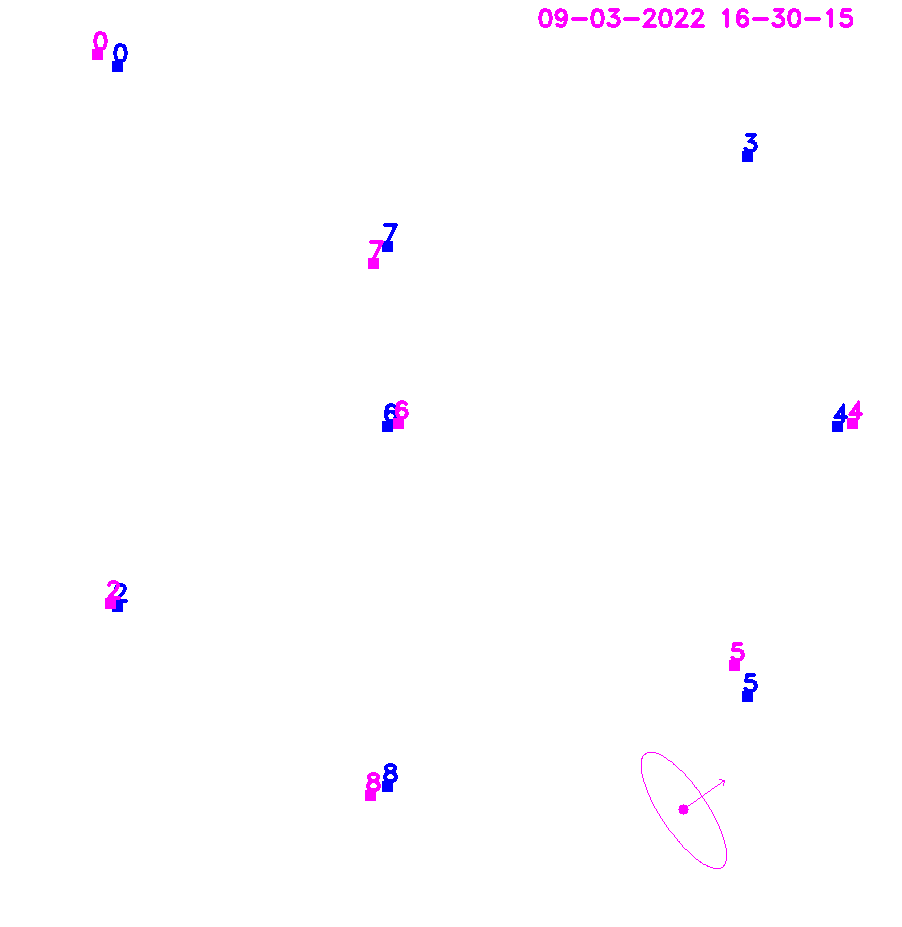
\includegraphics[width=6.5cm]{sample_run.png}
    \caption{Sample run of EKF SLAM}
    \label{fig:sample_run}
\end{figure}
    
\subsubsection{Parallelize covariance prediction} 

The parallelization of the covariance leads to four separate functions, \textit{GetTopLeft}, \textit{GetTopRight}, \textit{GetBottomLeft} and \textit{GetBottomRight}. Each one executed in one thread. The number of landmarks for this experiment was set to 10, which mainly influences the size of the matrix computation.

The average time for the multithreaded case averaged to 0.15ms while the sequential run was an order of magnitude lower at 0.0125ms. Varying the number of landmarks was limited by the Eigen C++ library to 100, which made the change in performance barely noticeable for having more or less landmarks. 

\subsubsection{Parallelize measurement prediction jacobian} 
The measurement prediction jacobian was parallelized by separating different landmark observations into different threads. As the computation is performed in constant time, the runtime reduction is not noticeable without a modification to the code. 

A 10ms delay was added to each landmark computation, simulating the process of matching and association in a real world system. 

At maximum, six observations were made at the same time by the robot, so having a feature batch size of one is reasonable for an eight core CPU. 

Perfroming the operations sequentially lead to the addition of the runtimes for each landmark. If the robot observes 6 landmarks, the delay is 60.3ms, if it observes 2 landmarks, the delay is 20.3ms.

However, parallelization improved this by dividing all the work into multiple threads, thus taking always 10.3ms no matter how many landmarks are seen. 

\subsubsection{Results and discussion}

Table \ref{table:res} shows the results mentioned earlier, demonstrating the two sides of multithreaded programming. It can be observed how thread creation is expensive. Spawning multiple threads for small problems reduces efficiency by increasing throughput. Meanwhile, computations that require time such as feature matching and detection in a robot SLAM system can be spread across multiple threads. In such a case, an increase in throughput also means an increase in performance. 

\begin{table}[!h]
\begin{tabular}{|l|l|l|}
\hline
\textbf{} & \textbf{$\Sigma_t^-$ Computation (ms)} & \textbf{$H_t$ Computation (ms)} \\ \hline
\textbf{Single thread}          & 0.0125                                                                & n of observations * 10.3       \\ \hline
\textbf{Multi thread}           & 0.12                                                                  & 10.3                           \\ \hline
\end{tabular}\caption{\label{table:res}Experiment Results} 
\end{table}

\section{Conclusion}
All in all, this report has provided a practical view of how to implement threads and shared memory in C++. It has studied the available options for multithreaded programming with practical examples, and finally demonstrated how it can be used in a robot localization and mapping system. It has also explored how multithreading, apart from requiring good knowledge on implementation to avoid deadlocks and races, can be detrimental if the application is not suitable for it, as well as beneficial for other scenarios. Further research in the topic would include to explore the other concurrent programming areas on atomic operations and abstraction levels. 


    
    

\addtolength{\textheight}{-12cm}   % This command serves to balance the column lengths
                                  % on the last page of the document manually. It shortens
                                  % the textheight of the last page by a suitable amount.
                                  % This command does not take effect until the next page
                                  % so it should come on the page before the last. Make
                                  % sure that you do not shorten the textheight too much.

%%%%%%%%%%%%%%%%%%%%%%%%%%%%%%%%%%%%%%%%%%%%%%%%%%%%%%%%%%%%%%%%%%%%%%%%%%%%%%%%
\newpage
\bibliographystyle{IEEEtran}  
\bibliography{IEEEbib}

\end{document}
